\documentclass{beamer}
\usetheme{JuanLesPins}

\usepackage[utf8]{inputenc}
\usepackage{latexsym}
\usepackage{amsmath, amsfonts, amssymb}
\usepackage{booktabs}
\usepackage{hyperref}

\newtheorem{defi}{Definición}[section]
\newtheorem{teor}{Teorema}[section]

\newcommand{\argmin}{\operatornamewithlimits{arg\ min}}
\newcommand{\normleft}{\left|\left|}
\newcommand{\normright}{\right|\right|}


\addtobeamertemplate{footline}
{%
   \usebeamercolor[fg]{author in sidebar}
   \vskip-1cm\hskip10pt
   %\insertpagenumber\,/\,\insertpresentationendpage\kern1em\vskip2pt%
   \insertframenumber\,/\,\inserttotalframenumber\kern1em\vskip2pt%
}


\title{Aplicación de la descomposición en valores singulares al análisis de datos}
\institute{Tutora: Amparo Baíllo Moreno\\\vskip 0.3cm Trabajo de Fin de Grado\\Doble Grado en Ingeniería Informática y Matemáticas\\Universidad Autónoma de Madrid}
\author{David Moreno Maldonado}
\date{2 Junio, 2020}

\begin{document}

\begin{frame}
\titlepage
\end{frame}
\begin{frame}{}
    \textcolor{red}{
    Esta presentación es una adaptación con los comentarios por escrito a la presentación en vídeo que se puede ver en \url{https://www.youtube.com/watch?v=fRixWFnNtB0}. Los comentarios extra aparecerán a lo largo de la presentación en este mismo color y, en general, sirven para aclarar y comentar los resultados obtenidos a lo largo del trabajo y que se comentan de manera oral en el vídeo.
    \vskip 0.5cm
    Se recomienda encarecidamente la visualización del mismo en vez de esta presentación en caso de ser posible y únicamente usar esta presentación como último recurso.}
\end{frame}

\begin{frame}
    \tableofcontents
\end{frame}

\section{Introducción}
\subsection{Objetivos del Trabajo de Fin de Grado}
\begin{frame}{}
\begin{itemize}
    \item Nuestra capacidad de recolectar y almacenar grandes cantidades de datos observados ha aumentado enormemente.

    \item Reducir la dimensión de los datos puede facilitar el análisis de la información muestral.

    \item La descomposición en valores singulares (SVD) es una técnica que permite resumir y comprimir la información contenida en la matriz de datos.

    \item Las técnicas estudiadas que hacen uso de la SVD son:
    \begin{itemize}
        \item Componentes principales.
        \item Correlaciones canónicas.
        \item Aproximación y compleción de matrices.
    \end{itemize}

    \item Se ha estudiado la base teórica detrás de cada una de las técnicas y, después, se han aplicado en datos reales y actuales.
\end{itemize}
\end{frame}

\subsection{Notación: Descomposición en valores singulares}
\begin{frame}{}
\begin{defi}
La \textbf{descomposición en valores singulares} (SVD) de una matriz $\mathbf{A}$ de dimensiones $m \times n$ es la factorización
$$\mathbf{A}=\mathbf{UDV}'$$ 
donde:
\begin{itemize}
    \item $\mathbf{U}$ es una matriz $m \times n$ ortogonal ($\mathbf{U}'\mathbf{U}=\mathbf{I}_n$) cuyas columnas $\mathbf{u}_j \in \mathbb{R}^m$ son los autovectores ortonormales de $\mathbf{AA'}$;
    \item $\mathbf{V}$ es una matriz $n \times n$ ortogonal ($\mathbf{V}'\mathbf{V}=\mathbf{I}_n$) cuyas columnas $\mathbf{v}_j \in \mathbb{R}^n$ son los autovectores ortonormales de $\mathbf{A'A}$;
    \item $\mathbf{D}$ es $n \times n$ y diagonal, cuyos componentes de la diagonal $\sigma_1 \geq \sigma_2 \geq \cdot \cdot \cdot \geq 0$ son los valores singulares de la matriz.
\end{itemize}
\end{defi}

Los valores singulares de $\mathbf{A}$ que son no nulos coinciden con la raíz cuadrada de los autovalores no nulos de $\mathbf{A'A}$ o $\mathbf{AA'}$.
\end{frame}

\section{Componentes principales}
\subsection{Base teórica}
\begin{frame}{Componentes principales}
\begin{defi}
    Las \textbf{componentes principales} de una matriz de datos $\mathbf{X}$ con $n$ observaciones p-variantes son las combinaciones lineales incorreladas $\mathbf{Y}_1 = \mathbf{Xt}_1, \ldots, \mathbf{Y}_p = \mathbf{Xt}_p$
    tales que la varianza muestral de cada $\mathbf{Y}_i$ es máxima condicionado a $\mathbf{t}_i'\mathbf{t}_i = 1$ y a que $\mbox{cov}(\mathbf{Y}_i, \mathbf{Y}_j) = 0$ para todo $j < i$
\end{defi}

Utilizamos la descomposición espectral, un caso particular de la SVD para matrices simétricas, para determinar de las componentes principales.
\begin{teor}
    Dada la matriz de covarianzas muestral $\mathbf{S}$ de la matriz de datos $\mathbf{X}$, si obtenemos su descomposición espectral $\mathbf{S = UDU'}$, las componentes principales de $\mathbf{X}$ son las combinaciones lineales $\mathbf{Y} = \mathbf{XUD}$.
\end{teor}
    
\end{frame}

\subsection{Aplicación a medidas biométricas de diferentes tipos aves}
\begin{frame}{Descripción de los datos}
\begin{itemize}
    \item Se disponen un total de 413 observaciones de diferentes tipos de aves.
    \item Las medidas disponibles se corresponden a la longitud y el diámetro de estos huesos:
    \begin{columns}
    \begin{column}{0.1\textwidth}
    \end{column}
    \begin{column}{0.5\textwidth}
    \begin{itemize}
        \item Húmero
        \item Cúbito
        \item Fémur
        \item Tibiotarso
        \item Tarsometatarso
    \end{itemize}
    \end{column}
    \begin{column}{0.4\textwidth}
    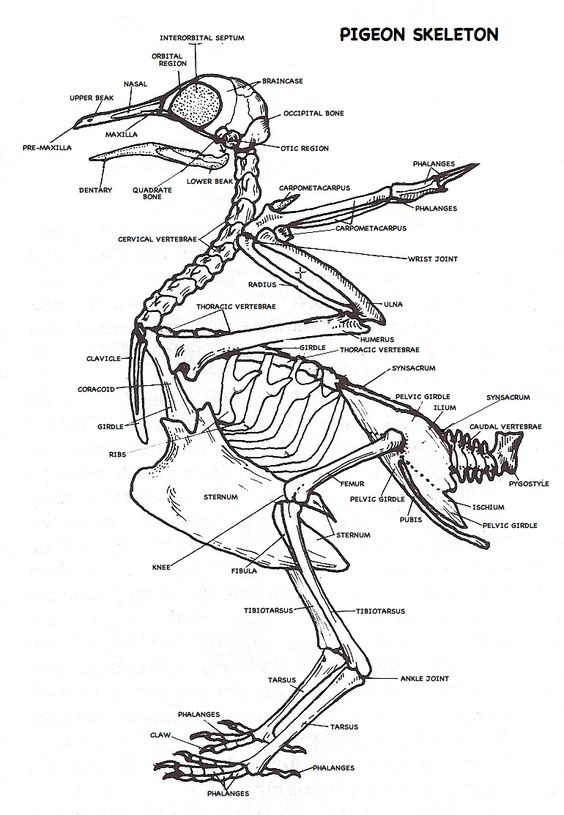
\includegraphics[scale=0.1]{img/bird.jpg}
    \end{column}
    \end{columns}
    \vskip 0.5cm
    \item Se realizará un análisis por separado de las longitudes y de los diámetros.
\end{itemize}
\end{frame}


\begin{frame}{Resultados longitudes de los huesos}
\textbf{Criterio del porcentaje:} Dados los porcentajes acumulados que cada componente principal $\mathbf{Y}_i$ explica de la variabilidad total, $P_i =  100 \frac{\sigma_1 + \cdots + \sigma_m}{\sigma_1 + \cdots + \sigma_p}$; podemos especificar un porcentaje $r$ y tomar las $m$ primeras componentes principales tal que $P_m > r$
\vskip 0.4cm
\scalebox{.85}{
\begin{table}
    \begin{tabular}{lccccc}
        \toprule \textbf{Variable} & \textbf{CP1} & \textbf{CP2} & \textbf{CP3} & \textbf{CP4} & \textbf{CP5}\\
        \midrule
        Húmero &  0.602 & -0.200 &  0.472 & -0.266 & -0.551\\
        Cúbito & 0.649 & -0.434 & -0.369 &  0.304 &  0.403\\
        Fémur &  0.187 &  0.257 & -0.674 & -0.649 & -0.154\\
        Tibiotarso & 0.375 &  0.668 &  0.351 & -0.117 &  0.525\\
        Tarsometatarso &  0.202 &  0.509 & -0.250 &  0.635 & -0.484\\
        \midrule Porcentaje de variación & 89.81\% &  7.98\% &  1.19\% & 0.68\% & 0.31\%\\
        Porcentaje acumulado & 89.81\% &  97.79\% &  98.99\% & 99.68\% & 100\%\\
        %Varianza escalada & 2.056 & 0.723 & 0.416 & 0.255 & 0.111\\
        \bottomrule
    \end{tabular}
\end{table}
}
\vskip 0.2cm
\textcolor{red}{Comentarios sobre estos resultados en la siguiente transparencia}
\end{frame}

\begin{frame}{Comentarios resultados longitudes de los huesos}
\begin{footnotesize}
\begin{enumerate}
\color{red}
    \item Existen diferentes criterios para decidir que componentes principales seleccionamos. En nuestro caso, utilizamos el criterio del porcentaje con un umbral del 95\%, seleccionando así las dos primeras componente principales.
    \item Podemos aplicar en este caso el teorema de Perron, estudiado en la memoria. Este dice que al aplicar componentes principales a una matriz totalmente positiva (como la matriz de covarianzas de las longitudes de los huesos) la primera componente principal será enteramente positiva y será la única que cumpla esto.
    \item La primera componente principal es la componente de tamaño y vemos que es más significativo el tamaño de los huesos de las alas (húmero y cúbito) que el de los de las patas (fémur, tibiotarso y tarsometatarso).
    \item La segunda componente es la de forma ya que contrapone las medidas de los huesos de las alas con los de las patas.
\end{enumerate}
\end{footnotesize}
    
\end{frame}



\subsection{Aplicación a medidas de células relacionadas con el cáncer de mama}
\begin{frame}{Descripción de los datos}
Imágenes digitalizadas de biopsias de senos. Las medidas tomadas se corresponden con el núcleo celular y son las siguientes:
\begin{minipage}[t]{0.48\linewidth}
   \begin{itemize}
        \item Radio: Media de las distancias del centro al perímetro.
        \item Textura: Desviación estándar de la escala de grises de la imagen.
        \item Perímetro.
        \item Área.
        \item Suavidad: Variación local de la longitud del radio.
    \end{itemize}
\end{minipage}
\begin{minipage}[t]{0.48\linewidth}
    \begin{itemize}
    \item Compacidad: $\frac{\mathrm{perimetro}^2}{\mathrm{area}-1}.$
    \item Concavidad: Agudeza de las porciones cóncavas del contorno.
    \item Puntos de concavidad: Número de porciones cóncavas del contorno.
    \item Simetría.
    \item Dimensión fractal.
    \end{itemize}
\end{minipage}
\end{frame}

\begin{frame}{Aplicación de la transformación por componentes principales de células malignas.}
\centering
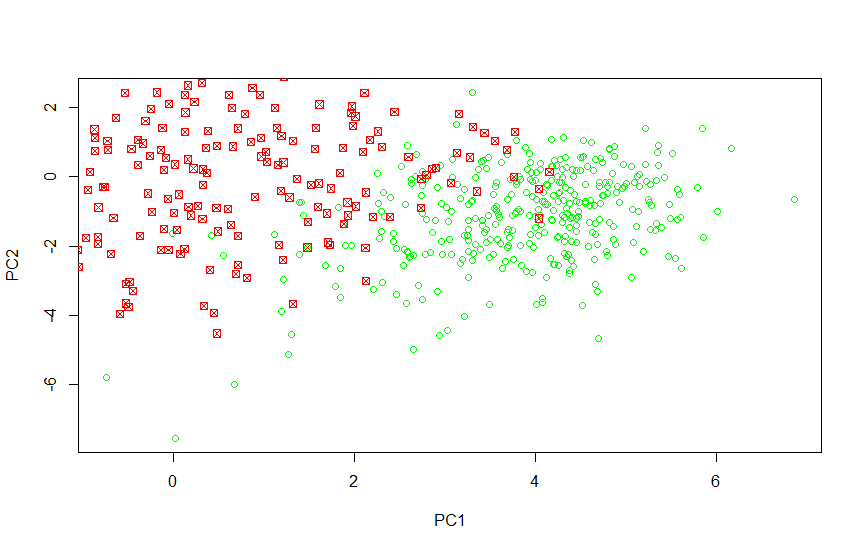
\includegraphics[scale=0.4]{img/breast_m}
\textcolor{red}{Comentarios sobre estos resultados en la siguiente transparencia}
\end{frame}

\begin{frame}{Comentarios resultados medidas de células}
\begin{footnotesize}
\begin{enumerate}
\color{red}
    \item Realizando un análisis por componentes principales para las células malignas análogo al de las medidas biométricas de aves, diferenciamos también dos componentes principales: la de tamaño y la de forma, que diferencia entre células redondeadas u onduladas.
    \item Aplicamos la transformación por componentes principales a todo el conjunto de datos y mostramos en verde las células benignas y en rojo las células malignas.
    \item En el gráfico se puede apreciar que existe una tendencia que puede permitir separar las benignas de las malignas y detectarlas en función de su tamaño y forma.
    \item Se realiza un proceso análogo con resultados similares para el análisis por componentes principales de las células benignas.
\end{enumerate}
\end{footnotesize}
    
\end{frame}


\section{Correlaciones canónicas}
\subsection{Base teórica}
\begin{frame}{Correlaciones canónicas (1/2)}
Sean $\mathbf{X}$ e $\mathbf{Y}$ dos matrices $n  \times p$ y $n \times q$, respectivamente, de observaciones de dos vectores en una muestra de $n$ individuos. Existen $m = \min (p,q)$ pares de vectores canónicos $\mathbf{a}_1, \mathbf{b}_1, \ldots, \mathbf{a}_m, \mathbf{b}_m$ que proporcionan:
\begin{align*}
\begin{array}{ccc}
    U_1 = \mathbf{Xa}_1, & V_1 = \mathbf{Yb}_1, & r_1 = \mbox{cor}(U_1,V_1)\\
    \vdots & \vdots & \vdots\\
    U_m = \mathbf{Xa}_m, & V_m = \mathbf{Yb}_m, & r_m = \mbox{cor}(U_m,V_m)\\
\end{array}
\end{align*}
de tal manera que cada $r_i$ es máxima en cada caso y $\mbox{cor}(U_i, U_j)=0$ y $\mbox{cor}(V_i, V_j)=0$ para todo $j<i$. 

Cada par de $U_i$ y $V_i$ definen las i-ésimas \textbf{variables canónicas} y cada $r_i$ es la i-ésima \textbf{correlación canónica}.
\end{frame}


\begin{frame}{Correlaciones canónicas (2/2)}
Denotamos $\mathbf{S}_{11}$ y $\mathbf{S}_{22}$ las matrices de covarianzas muestrales de $\mathbf{X}$ e $\mathbf{Y}$, respectivamente. Y las matrices de covarianzas cruzadas $\mathbf{S}_{12} = \mathbf{S}_{21}'$.
Consideramos la matriz $p \times q$:
\begin{equation*}
    \mathbf{Q} = \mathbf{S}_{11}^{-1/2}\mathbf{S}_{12}\mathbf{S}_{22}^{-1/2},
\end{equation*}\\
Sea $\mathbf{Q = UDV'}$ la descomposición en valores singulares de esta matriz.
\begin{teor}
    Los vectores canónicos y correlaciones canónicas son
    \begin{equation*}
        \mathbf{a}_i = \mathbf{S}_{11}^{-1/2}\mathbf{u}_i,\ \  \mathbf{b}_i = \mathbf{S}_{22}^{-1/2}\mathbf{u}_i,\ \  r_i = \sigma_i,
    \end{equation*}
    donde $\mathbf{u}_i$ son las columnas de $\mathbf{U}$ y $\mathbf{D} = \mbox{diag}(\sigma_1, \sigma_2, \ldots)$ con $\sigma_i \geq \sigma_{i+1}$ para todo $i$.
\end{teor}
    
\end{frame}

\subsection{Aplicación a índices de nivel educativo y libertad de las mujeres de diferentes países}
\begin{frame}{Índices sobre el nivel educativo}
\begin{footnotesize}
\textcolor{red}{Aplicamos el análisis de correlaciones canónicas a dos grupos de variables: indicadores del nivel educativo en esta transparencia e índices de las libertades y derechos de la mujer en la siguiente.}
\begin{itemize}
    \item ALF-JOVEN = Ratio de alfabetismo en mujeres jóvenes (\% de mujeres entre 15 y 24 años).
    \item ALF-ADULTA = Ratio de alfabetismo en mujeres adultas (\% de mujeres mayores de 15 años).
    \item EST-PROF-PRIM = Ratio estudiante-profesor en educación primaria.
    \item EST-PROF-SEC = Ratio estudiante-profesor en educación secundaria.
    \item INSC-PRIM = Porcentaje de inscripción femenino en educación primaria.
    \item INST-SEC = Porcentaje de inscripción femenino en educación secundaria.
    \item PROFESORAS = Porcentaje de profesoras en la educación secundaria.
\end{itemize}
\end{footnotesize}
\end{frame}

\begin{frame}{Índices sobre los derechos y libertades de las mujeres}
Indican el porcentaje de mujeres que creen que está justificado que su marido la golpee si:
\begin{itemize}
    \item Ella discute con él. (DISCUTIR)
    \item A ella se le quema la comida.(COMIDA)
    \item Ella desatiende a los hijos. (HIJOS)
    \item Ella sale de casa sin consultárselo. (SALIR)
    \item Ella se niega a mantener relaciones sexuales con él. (RELACIONES)
\end{itemize}
\end{frame}

\begin{frame}{Resultados de la aplicación de correlaciones canónicas}
\begin{columns}
\begin{column}{0.5\textwidth}
\scalebox{.8}{
\begin{table}
    \begin{tabular}{lcc}
        \toprule \textbf{Variable} & \textbf{CC1} & \textbf{CC2}\\
        \midrule
        ALF-JOVEN & -0.023 & -0.030\\
        ALF-ADULTA & 0.009 &  0.019\\
        EST-PROF-PRIM & 0.006 & -0.010\\
        EST-PROF-SEC & 0.004 &  0.007\\
        INSC-PRIM & -0.002 &  0.011\\
        INSC-SEC & 0.008 &  0.000\\
        PROFESORAS & -0.001 &  0.006\\
        \midrule DISCUTIR & -0.027 & -0.028\\
        COMIDA & 0.032 &  0.010\\
        HIJOS & -0.031 &  0.001\\
        SALIR & 0.040 &  0.024\\
        RELACIONES & -0.002 & -0.019\\
        \midrule \textbf{Correlación canónica} & 0.928 & 0.856\\
        \bottomrule
    \end{tabular}
\end{table}
}
\end{column}

\begin{column}{0.5\textwidth}
\begin{footnotesize}
\begin{enumerate}
    \color{red}
    \item Existe una correlación muy alta entre estos dos grupos de variables, muestra de ello es el alto valor que alcanzan la primera y la segunda correlación canónica.
    \item Podemos destacar el papel de la alfabetización de las mujeres jóvenes dado el peso que obtiene esta variable en ambas variables canónicas.
\end{enumerate}
\end{footnotesize}
\end{column}

\end{columns}

\end{frame}


\section{Aproximación y compleción de matrices}
\subsection{Base teórica}
\begin{frame}{Problema aproximación de matrices}
Sea una matriz $\mathbf{A}$ de dimensiones $m \times n$, el problema de optimización para aproximarla es
\begin{equation*}
    \hat{\mathbf{A}} =\argmin_{\mathbf{M} \in \mathbb{R}^{m \times n}} \| \mathbf{A} - \mathbf{M} \|^2 \mathrm{\ sujeto\ a\ }\Phi(\mathbf{M}) \leq c,
\end{equation*}
donde la función $\Phi$ sirve para establecer una restricción que hace que la matriz $\hat{\mathbf{A}}$ tenga muchos ceros (\textit{sparse}).
\end{frame}

\begin{frame}{Teorema de la aproximación}
\begin{teor}
    Dada una matriz $\mathbf{A}$ de dimensiones $m \times n$, la matriz de rango menor o igual que $k$ (expresada en la forma $\sum_{i=1}^{k} \mathbf{x}_i \mathbf{y}_i'$)
    que mejor aproxima a $\mathbf{A}$, en el sentido de que minimiza el error de aproximación
    \begin{equation*}
        \normleft \mathbf{A} -  \sum_{i=1}^{k} \mathbf{x}_i \mathbf{y}_i' \normright
    \end{equation*}
    donde $\normleft \mathbf{A} \normright$ es la norma de Frobenius de $\mathbf{A}$, viene dada por los $k$ primeros términos de la SVD de la matriz $\mathbf{A}$, $\mathbf{A}_k$.
\end{teor}

Resolvemos el problema de la aproximación tomando:
\begin{equation*}
    \mathbf{M} = \mathbf{A}_k,\  \Phi(\mathbf{M}) = \mbox{rank}(\mathbf{M}) \mathrm{\ y\ } c = k \leq \mbox{rank}(\mathbf{A})
\end{equation*}
\end{frame}

\begin{frame}{Problema de compleción de matrices}
Sea $\mathbf{A}$ la matriz con datos en un subconjunto $\Omega \subset \{1, \ldots, m\} \times \{1, \ldots, n\}$ y $\textbf{M}$ una aproximación,  el problema de optimización para la compleción de matrices es
\begin{equation*}
    \min_{\mbox{rank}(\mathbf{M}) \leq r} \sum_{(i,j) \in \Omega} (a_{ij} -  m_{ij})^2.
\end{equation*}
\begin{itemize}
    \item El problema es no convexo y las soluciones globales no son posibles de manera general.
    \item Existen heurísticas que permiten encontrar mínimos locales de manera efectiva utilizando una estimación inicial.
\end{itemize}
    
\end{frame}

\begin{frame}{Algoritmo iterativo del paquete \texttt{SoftImpute} de R para compleción de matrices}
Sea $\mathbf{A} = (a_{ij})$ la matriz con datos observados en un subconjunto $\Omega \subset \{1, \ldots, m\} \times \{1, \ldots, n\}$, $\mathbf{M} = (m_{ij})$ una estimación inicial de los valores faltantes de $\mathbf{A}$ y $P_\Omega (\mathbf{A})$ la matriz con los valores de $\Omega$ mantenidos como en $\mathbf{A}$ y el resto igualados a $0$. El algoritmo seguido es:
\begin{enumerate}
    \item $\mathbf{Z} = P_\Omega(\mathbf{A}) + P_{\Omega^{\bot}}(\mathbf{M})$
    \item Hallamos la SVD $\mathbf{Z=UDV'}$
    \item Obtenemos la matriz $\mathbf{D}_k$, igual a la matriz $\mathbf{D}$, pero igualando a cero todos los valores singulares que no sean los $k$ primeros.
    \item Construimos $\mathbf{Z}_k=\mathbf{UD}_k\mathbf{V'}$
    \item Actualizamos la matriz $\mathbf{M=Z}_k$
\end{enumerate}
\end{frame}

\subsection{Aplicación de la compleción de matrices}
\begin{frame}{Datos de películas utilizados}
\scalebox{.7}{
\begin{table}
    \begin{tabular}{ccccccc}
        \toprule
        \textbf{Pulp} & \textbf{Los juegos} &  & \textbf{El corredor} & \textbf{El lobo de} & \textbf{El viaje} &\\
        \textbf{fiction} & \textbf{del hambre} & \textbf{Interestellar} & \textbf{del laberinto} & \textbf{Wall Street} & \textbf{de Chihiro} & \textbf{Seven}\\
        \midrule
        4 & 3 & 5 & 2 & 4 & 5 & 5\\
        4 & 2 & 5 & 2 & 5 & 4 & 4\\
        5 & 3 & 5 & 3 & 4 & 4 & 4\\
        3 & 3 & 5 & 2 & 4 & 5 & 4\\
        4 & 3 & 1 & 1 & 3 & 4 & N/A\\
        4 & 3 & N/A & N/A & 3 & 4 & 4\\
        5 & 2 & 5 & 2 & 4 & 5 & 5\\
        4 & 3 & 5 & 3 & 4 & 3 & 3\\
        5 & 3 & 4 & 1 & 3 & 4 & 4\\
        4 & 2 & 5 & 4 & N/A & 5 & N/A\\
        4 & 4 & 4 & 4 & 4 & 4 & 4\\
        5 & 4 & 5 & N/A & 5 & 5 & 5\\
        5 & 1 & 4 & N/A & 4 & N/A & 4\\
        \bottomrule
    \end{tabular}
\end{table}
}
\vskip 0.3cm
\textcolor{red}{Comentarios sobre esta tabla en la siguiente transparencia}
    
\end{frame}

\begin{frame}{Comentarios sobre la aplicación de \textt{SoftImpute}}
\begin{enumerate}
    \color{red}
    \item Se pretende realizar una recreación a menor escala del famosos problema de Netflix para crear un recomendador de contenido. Se puede consultar en profundidad en la memoria.
    \item Se han recopilado datos de diferentes péliculas mediante su valoración entre 1 y 5 puntos.
    \item Existen datos faltantes (N/A) y hemos añadido más eliminando algunos de los observados. De esta manera, podemos observar como de buena es la aproximación obtenida.
\end{enumerate}
    
\end{frame}

\begin{frame}{Resultados de la aplicación de \texttt{SoftImpute}}
\scalebox{.75}{
\begin{table}
    \begin{tabular}{cccccc}
        \toprule
        \textbf{Rango} & \textbf{Iteraciones} & \textbf{Diferencia} & \textbf{Diferencia} & \textbf{Diferencia} & \textbf{Diferencia}\\
        \textbf{máximo} & \textbf{hasta convergencia} & \textbf{total} & \textbf{media} & \textbf{mínima} & \textbf{máxima} \\
        \midrule
        1 & 6 & 8.505 & 1.063 & 0.288 & 1.891\\
        2 & 12 & 17.157 & 2.145 & 0.254 & 6.112\\
        3 & 26 & 19.073 & 2.384 & 0.052 & 7.626\\
        4 & 24 & 29.593 & 3.699 & 0.248 & 6.662\\
        5 & 50 & 27.593 & 3.449 & 1.234 & 6.491\\
        6 & 15 & 30.165 & 3.771 & 0.661 & 6.542\\
        \bottomrule
    \end{tabular}
\end{table}
}
\vskip 0.3cm
\textcolor{red}{En este ejemplo, la mejor aproximación se consigue usando una restricción de rango igual a 1. No solo se consigue con esto que el algoritmo converja en el menor numero de iteraciones, sino que la diferencia total con la matriz observada (siendo esta la distancia de Frobenius) es la menor de todos los rangos probados.}
\end{frame}

    
%\end{frame}
\begin{frame}{}
  \centering \huge
  \emph{Muchas gracias.}
\end{frame}
\end{document}